\chapter{Measurement Setup \& Techniques} \label{chapter:measurement}

In this chapter we discuss the measurement setup and techniques used in our experiments. Our setup consists of the qubit chip presented in chapter \ref{chapter:design}, held at the 20~mK stage of a He$_3$/He$_4$ dilution refrigerator and connected to a signal generation and measurement chain including cryogenic microwave components and room temperature electronics. We describe how the processor chip is mounted, as well as the individual parts of the signal  and measurement chain, putting emphasis on microwave pulse generation. Afterwards we discuss the calibration and compensation techniques that we use to correct signal imperfections when generating qubit drive and flux signals. Finally we introduce the different measurement protocols used for driving and reading the qubit, as well as for determining all relevant qubit parameters such as frequency, anharmonicity, and relaxation and dephasing times.

\smallskip

\section{Chip Mounting}

\begin{SCfigure}[1][ht!]
	\centering
		\includegraphics[width=0.6\textwidth]{"./material/photos/sample holder/sample_holder"}
	\caption[]{Chip mounting. Complete sample-holder (a), cover part as seen form below (b), and bottom part (c) with the mounted PCB carrying the qubit chip and the mini-SMP connectors. (d)  chip  wire-bonded to the PCB. Wire bonds to four CPW lines can be seen on the top and bottom of the picture, as well as on-chip bond wires reconnecting separated grounds inside the chip. The whole sample holder is screwed to the 20~mK stage of the dilution refrigerator.}
	\label{fig:pcb_and_sample_holder}
\end{SCfigure}

Chip mounting is illustrated in  fig. \ref{fig:pcb_and_sample_holder}. The chip is first attached to the lower part of the sample holder using wax (melting temperature 80°C). It is placed in a groove whose depth matches the height of the silicon chip, such that the top part of it is at the level of the surface of the sample holder after mounting. We use six small microwave PCBs, each equipped with a $50\;\Omega$ coplanar waveguide and a right-angle mini-SMP connector, which are also placed in matched grooves on the sample holder, as shown in fig. \ref{fig:pcb_and_sample_holder}c. The PCBs are made of TMM10 with a dielectric constant of 10 close to that of the silicon chip. They are metalized on both sides with gold-coated copper and have vias to connect the metal layers on both sides. The three electrodes of each CPW line on the chip are wire-bonded to their counterparts on the PCBs using aluminum wires of 50 µm diameter. In addition, on-chip bond wires are used to reconnect separated parts of the ground plane that are initially isolated from each other because of the circuit topology, as shown in fig. \ref{fig:pcb_and_sample_holder}d. This is important in order to avoid spurious on-chip resonances in the relevant frequency window, i.e. below 10 GHz \citep{schuster_circuit_2007}.

The lower part of the sample holder with the chip and the small PCBs is then mounted to the gold-coated top part as shown in fig. \ref{fig:pcb_and_sample_holder}a/b, which thermally anchors the chip to the mixing chamber of the refrigerator, shields it from electromagnetic noise and encloses it in a conducting cavity that is small enough to suppress box resonances in the relevant frequency window. Grooves in the top part of the sample holder, shown in fig. \ref{fig:pcb_and_sample_holder}b, provide the necessary open space above the qubit chip and the six coplanar waveguides.

The whole sample-holder is mounted in the refrigerator by screwing it around a small coil that sits inside the cover and produces a DC magnetic field perpendicular to the chip. The distance between the chip and the lower end of the coil is less then 3 mm.

\section{Signal Generation \& Acquisition}

\begin{figure}[ht!]
	\centering
		\includegraphics[width=1.\textwidth]{"./material/figures/2-qubit-processor/measurement setup"}
	\caption[The measurement setup used for the two-qubit experiments]{Measurement setup used for the two-qubit experiments. The very same drive and readout setup is used for both qubits, so that only one exemplary is shown. The role of each line is indicated on top, and  the relevant parameters indicated beside each component, including the wire and cable materials. Elements shown are attenuators, low pass or bandpass filters, circulators and isolators, microwave amplifiers, IQ mixers, microwave and arbitrary waveform generators,and an acquisition board and a spectrum analyzer. }
	\label{fig:measurement_setup}
\end{figure}

Figure \ref{fig:measurement_setup} shows the wiring of our experiment from room temperature down to the 20~mK stage. Except for the small coil that is shared by both qubits, the rest of the circuitry is duplicated for each of them and only one exemplary is shown on the figure. One can see the bifilar dc flux line and a fast coaxial 50~$\Omega$ flux line on the left, as well as a set of 50~$\Omega$ coaxial microwave drive and readout lines on the right. Lossy cables or wires made from special alloys such as CuNi, CuBe, stainless steel (SS) and manganin are used at intermediate temperatures, as needed for minimizing the heat transfer between the different stages. Between 20~mK and 4~K, superconducting NbTi cables are used for the measurement lines because they have both a low thermal conductivity and a low microwave attenuation. Semi-flexible Copper microwave coaxial cables are used at 20~mK.

\subsection{Driving and Measurement of the Qubits}

Each of the qubits together with its corresponding readout resonator is fitted with an individual fast flux , drive, and measurement circuit. The microwave and arbitrary waveform generators used to control the experiment, as well as the acquisition systems, are all phase-locked using 10MHz external clocking.
At room temperature we generate qubit and readout resonator drive waveforms using phase-locked single-tone microwave sources whose continuous output is mixed with control pulses generated by two arbitrary waveform generators (more details in the next section). The qubit drive and readout drive signals are then combined on a single line and sent to the chip through a series of cryogenic attenuators and filters. A cryogenic circulator at 20~mK routes the incoming pulses to the qubit chip, where they are sent to the qubit readout resonator and finally reflected by it. The reflected signal passes again through the circulator and gets routed through a double isolator and a band-pass filter to a cryogenic high electron mobility amplifier (HEMT) with a gain of 40~dB. The amplified signal gets then transmitted to the room temperature electronics, where it is filtered and amplified further by more then 50~dB. Finally, the signal is demodulated using a two-quadrature mixer and a continuous microwave reference tone (local oscillator), the two resulting quadrature being further amplified, filtered below 200MHz and  fed to two channels of  a 4-channel ADC board. Flux pulses are generated using an arbitrary waveform generator at room temperature. The signal is then sent to the qubit chip through a 20~dB attenuator, through a Microtronics low-pass filter of the reflective type with a 1.35 GHz frequency cutoff, and through a custom-made high-frequency powder filter that uses an absorptive material (Eccosorb) to attenuate high-frequency noise. After passing through the transmission line on the qubit chip, the outgoing flux signal is routed to room temperature electronics using a transmission line identical to the input line. There, the signal can be measured, which is useful for characterizing possible signal imperfections caused by the non-ideal character of the line.

\subsection{X-Y Pulse Generation by Microwave Single Sideband Mixing}

As briefly mentioned above, a single-sideband mixing technique is used to generate the qubit X and Y driving pulses. More precisely, each qubit has its own IQ mixer driven with a continuous single-frequency microwave tone and two synchronized intermediate frequency control signals generated by an arbitrary waveform generator (Tektronix AWG5014b). In general, when feeding a signal $LO(t) = I_0 \cos{(\omega_{LO} t )}$ to the LO port of an IQ mixer and two signals $I(t)$, $Q(t)$ to its I and Q ports, one obtains a signal

\begin{equation}
RF(t) = I(t)\cos{(\omega_{LO} t)}+Q(t)\sin{(\omega_{LO} t)} \label{eq:iqMixer}
\end{equation}
at the RF output port. (Since the IQ mixer that we use is a passive reciprocal device, one can as well feed two input signals to the LO and RF ports and obtain the demodulated signal quadratures at the I and Q ports after filtering, a technique that we make use of in our qubit readout scheme). Typically we use heterodyne single sideband mixing to generate driving pulses that are tunable in frequency with respect to the local oscillator (carrier  frequency), over the mixer bandwidth (several hundreds of MHz): Ideally, the I and Q signals should have the form $I(t)=s(t)\cos(\omega_{IF} t-\phi)$ and $Q(t)=s(t)\sin(\omega_{IF} t-\phi)$ in order to obtain an output pulse $RF(t)=s(t)\cos[(\omega_{LO}-\omega_{IF})t +\phi]$ that will induce a rotation of the qubit around axis $X_{\phi}$ laying in the equatorial plane of the Bloch sphere and making an angle $\phi$ with the $X$ axis. The phase reference of the driving pulses is thus defined by both the carrier phase and the common starting time of the I and Q waveforms with respect to the carrier. Both quantities have to be kept constant over subsequent sequences. In addition, when performing experiments on multiple qubits, the phase differences between the reference phases of each qubit must also be conserved.  We explain below in the section devoted to synchronization how these phase references are maintained. In the expression above $s(t)$ is the envelope of the pulse, the area of which defines the angle of rotation. For small rotation angle, we choose for $s$ a Gaussian shape of the form
%
\begin{equation}
s(t) = s_0\cdot\exp{\left[-\frac{(t-t_0)^2}{2\sigma_t^2}\right]}
\end{equation}
%
with "rise time" $\sigma_t=3\;\mathrm{ns}$ and a cutoff at $-3\sigma_t\le t-t_0\le 3\sigma_t$. The advantage of using such a Gaussian pulse \citep{bauer_gaussian_1984} is that its Fourier transform is again a Gaussian, which, in contrast to a rectangular pulse, does not exhibit side lobes in the frequency domain and thus minimizes the leakage to higher Transmon levels discussed in section \ref{section:charge_driving}. To increase the Rabi angle of such a pulse, we just change its amplitude as far as it does not saturate the IQ mixer. For larger Rabi angles we simply add a flat plateau between the Gaussian rise and fall.

\begin{figure}[ht!]
	\centering
		\includegraphics[width=0.7\textwidth]{"./material/figures/measurement/mixer_imperfections"}
	\caption[...]{Illustration of the method used to measure and correct the imperfect behavior of the IQ mixers used for  our heterodyne single-sideband generation of the qubit drives: the leakage of the LO signal to the RF port is measured continuously with a spectrum analyzer and is minimized by tuning the two offset voltages $I_0$ and $Q_0$ at the I and Q ports. To correct phase and amplitude errors during heterodyne mixing, we then add two sideband signals to the IF ports and minimize iteratively the measured RF power at $\omega_{LO}+\omega_{IF}$ by tuning the amplitude and phase of two correction waveforms added to the I and Q ports.}
	\label{fig:iq_mixer_correction}
\end{figure}

Commercially available IQ mixers are not perfect, and deviate from the ideal behavior given by eq. (\ref{eq:iqMixer}). Typical imperfections include large insertion losses --i.e. loss of  power between the different ports of the mixer--, RF signal leakage at zero IQ-input, and frequency-dependent phase and amplitude errors of the mixed sideband signals. In order to achieve reliable single-qubit operations we need to correct these errors, as shown in Fig. \ref{fig:iq_mixer_correction}. The signal leakage consists in a small part of the LO signal leaking through to the RF port even when the IQ inputs are zeroed. This leakage can be compensated by adding to the IQ ports DC offset voltages that depend on $\omega_{LO}$. The appropriate offsets can be determined by applying a continuous signal at a frequency $\omega_{LO}$ to the LO port and minimizing the measured signal power at the RF port. Using this method, the leakage power can be reduced down to -80 dBm.

To correct the sideband amplitude and phase errors we apply another correction procedure. We first introduce the notation
\begin{equation}
A(t) = I(t)+iQ(t) = a(t)\exp{[-i \phi(t)]} \label{eq:iq_if_input}
\end{equation}
for any composite I and Q signal. We then consider such a signal at a single sideband frequency $\omega_{IF}$ and at a fixed complex amplitude $a(t)=a= a_0\exp{(i\phi_0)}$ such that $A(t) =a \exp{[-i \omega_{IF} t]} $. The effect of the gain and phase imperfections are responsible for a spurious additional output signal at the mirrored sideband frequency $-\omega_{IF}$ with respect to the carrier. This unwanted signal would be obtained in a perfect mixer with an IQ signal $\varepsilon(\omega_{IF},\omega_{LO})A^*(t)$. We can thus remove it by adding a small correction $c(\omega_{IF},\omega_{LO})A^*(t)$ to our IQ input signal. The complex-valued correction coefficient $c(\omega_{IF},\omega_{LO})=|c|\exp{(i\;\mathrm{arg}[c])}$ usually depends both on the LO frequency $\omega_{LO}$ and the sideband frequency $\omega_{IF}$. We thus determine it  by generating a continuous single sideband at frequency  $\omega_{LO}-\omega_{IF}$  and by finding  iteratively the  $c(\omega_{IF},\omega_{LO})$ that minimizes the amplitude of the unwanted sideband at $\omega_{LO}+\omega_{IF}$, measured with a spectrum analyzer (see Figs.  \ref{fig:measurement_setup} and \ref{fig:iq_mixer_correction}). Both the offset and the sideband-amplitude and -phase corrections have been automated using our data acquisition software. By using this optimization techniques we can lower the amplitudes of the $\omega_{LO}$  and $\omega_{LO}+\omega_{IF}$ peaks down to 80 dB and 70 dB below the targeted sideband at $\omega_{LO}-\omega_{IF}$, respectively.

\smallskip

Finally, it is important to tolerate the maximum and minimum absolute ratings for the signals applied to the I/Q  as well as LO and RF ports of the mixer in order to avoid saturation and nonlinear response. For the mixer that we use in our setup (Hitite HMC 525), the maximum input powers are given as 20 dBm for the RF and I/Q ports and 27 dBm for the LO port. In addition, the maximum tolerable DC current of the mixer at the I/Q ports is limited to 3 mA, which restricts the DC offset voltage that we can supply to the mixer.

\subsection{Fast Magnetic Flux Pulse Generation and Calibration}

The fully symmetric coaxial line used for sending fast magnetic flux pulses to one of the qubits has been described above and is shown on Fig. \ref{fig:measurement_setup}. The low-pass filtering of the line is optimized to reduce high-frequency noise as much as possible while letting the line pass pulses with 2-3 ns rise time. Consequently, the pulse  distortion by the line is not negligible. Another important imperfection in our pulse generation is the finite bandwidth of the arbitrary waveform generator we use ( Tektronix AWG5014B). It is about 500~MHz and some ringing is observed at a few percent level for square pulses with rise times below 10 ns. For compensating all these imperfections, we measure the frequency response of each part of the whole circuit with our 1 GHz bandwidth acquisition system. A step function with 2 ns rise time and 1ns/sample is programmed on the AWG and measured at the output of the flux line. This allows us to obtain the response function of the generator (DAC) and of the input line. We then model the whole chain as shown on Fig. \ref{fig:FluxLineResponseFunction}a, using the same response function for the identical input and output lines. The Fourier transform of the measured signal at the end of the output line is given as

\begin{SCfigure}[1.0][ht!]
	\begin{tabular}{l}
	 a) \\ \includegraphics[width=0.5\textwidth]{"./material/figures/measurement/fluxline_model"} \\
	 b) \\ \includegraphics[width=0.6\textwidth]{"./material_thesis/fluxline response/response"} \\
	 c) \\ \includegraphics[width=0.6\textwidth]{"./data/ct5/2010_06_15 - fluxline response/test_measurement_modified"}
	 \end{tabular}
	 \caption[]{a) Schematic of the flux line chain used in our setup. The flux signal is generated by a DAC, fed through the input line to the sample, returned to room temperature through the output line and digitized by an ADC. b) Measured response functions of different parts of the flux line, showing the response of the DAC and ADC circuits and of the input part and the full flux line. c) Illustration of the signal correction method. We generate a desired waveform (in red) without applying any correction, measure the arriving signal at the sample (in magenta), calculate the response function of the line and generate a corrected signal (in green), which we measure again at the sample (in blue). The corrected signal corresponds to a good degree to the desired input signal.}
	 \label{fig:FluxLineResponseFunction}
\end{SCfigure}

%
\begin{equation}
\chi_{\mathrm{fl}}(\omega) = \chi_{signal}\cdot \chi_{DAC}\cdot \chi_{\mathrm{input}}\cdot\chi_{\mathrm{output}}\cdot\chi_{ADC}, \label{eq:flux_response}
\end{equation}
%
with $\chi_{\mathrm{signal}}$ the Fourier transform of the ideal input signal, $\chi_{ADC}$ and $\chi_{DAC}$ the response functions of the DAC and ADC (which we measure independently), and $\chi_{\mathrm{input}}=\chi_{\mathrm{output}}$ the response function of the input and output transmission lines. By measuring $\chi_{\mathrm{fl}}$, subtracting the ADC and DAC responses from it, we obtain the input line response function $\chi_{\mathrm{input}}$. To correct the signal distortion seen by the qubit, we can then simply re-program the AWG with a corrected wave function with Fourier transform 
%
\begin{equation}
\chi_{\mathrm{signal}}^{\mathrm{corr}} = \chi_{\mathrm{signal}}\cdot (\chi_{DAC}\cdot\chi_{\mathrm{input}})^{-1}\cdot \mathrm{G}(\omega,\omega_{co}).
\end{equation}
%
Here, $G(\omega,\omega_{co})$ is a Gaussian filter function with a cutoff frequency $\omega_{co}$ that we apply to the inverse measured response function to eliminate the distortion at high frequencies caused by the fact that we are not able to accurately measure the response function of the flux line above the bandwidth of our digitizing board. Usually, we set this cutoff frequency to $\omega_{co}/2\pi=400\;\mathrm{MHz}$, which allows us to correct most signal distortion in the frequency window relevant to this work, i.e. up to half a GHz. Figure \ref{fig:FluxLineResponseFunction}b shows the measured response functions of the flux line and fig. \ref{fig:FluxLineResponseFunction}c shows an exemplary measurement, where we first program an ideal waveform (in red) in the AWG, send it through the flux line, calculate the shape of the waveform at the sample (in magenta) by measuring the waveform at the output of the line and subtracting the measured response functions of the ADC and the output line, then program a corrected waveform (in green) and finally measure the shape of this waveform at the sample again (in blue), which now corresponds closely to the ideal waveform.
 


\smallskip

After having corrected the response of the flux line by this technique, we can further reduce signal distortion by directly probing the flux seen by the qubit at a given time. For this, we apply a small test flux signal $\phi_{ext}^{fl}(t)$ to the qubit, measure its frequency $\omega_{01}(t)$ and reconstruct the flux from the previously measured  $\omega_{01}(\phi_{ext})$ curve. If the qubit frequency is chosen well away from its maximum and minimum frequencies, i.e. where $\gamma=\partial \omega_{01}/\partial \phi_{ext}^{fl} \ne 0$, and if the flux signal is comparably small, the time-dependent qubit frequency is $\omega_{01}(t)=\omega_{01}^0+\gamma.\delta\phi_{ext}^{fl}(t)$. The frequency displacement of the qubit is thus proportional to the applied flux signal. Now, if we drive the qubit with a calibrated $X_\pi$ Rabi pulse at a given drive frequency $\omega_{d}$ at time $t_0$, the probability of finding it in state $\ket{1}$ afterwards is maximum if $\omega_{d}=\omega_{01}(t_0)$. Thus, by maximizing this probability as a function of $\omega_{d}$, we can reconstruct the flux $\phi_{ext}^{fl}(t_0)$ seen by the qubit at any given moment. Of course, the time resolution achieved with this method is limited to the pulse duration of the $X_\pi$ pulse, which is typical $3-5\;\mathrm{ns}$. After having reconstructed the flux signal $\phi_{ext}^{fl}(t)$ seen by the qubit, we can again calculate its Fourier transform and correct imperfections by further changing the input signal.

\subsection{Microwave and DC Pulse Synchronization}

In our experiment, each qubit possesses two microwave sources that generate the continuous tones for drive and readout. The two fast pulse signals mixed with the two driving tones of the two qubits are generated by a single 4-channel arbitrary waveform generator (Tektronix AWG5014B). A second AWG generates the flux pulses for the two qubits. The measurement of the reflected and demodulated readout signal of both qubits is done by a single ADC card. All these different signal generators and measurement devices need to be synchronized in order to keep the relative phases and time differences between them constant over successive individual runs of our experiment. For this, we use a 10 MHz frequency reference chain, whose master clock is generated by the AWG generating the qubit drive pulses. The reference signal is then passed on to all microwave sources and signal generators as well as oscilloscopes, spectrum analyzers and ADC cards in our setup. In addition, to avoid random phase-jitter between the signals of the two microwave sources that generate the drive pulses of the two qubits, their drive frequencies are chosen such that they correspond to a multiple of the repetition frequency of the master AWG, which is typically 50 kHz. When this condition is met, the relative phases between the two microwave signals is conserved between individual runs of an experiment, which is crucial when performing measurements sensitive to this phase such as quantum state tomography two entangled qubits. In addition, a 1 GHz phase synchronization chain is used to phase-lock the two microwave generators and reduce the phase drift between them.

\section{Measurement Techniques}

In this section, we discuss the techniques used to manipulate and characterize our two-qubit processor. We address qubit readout and describe how the relevant qubit parameters are determined.

\subsection{Qubit Readout} \label{section:qubit_readout}

\begin{figure}[ht!]
\centering
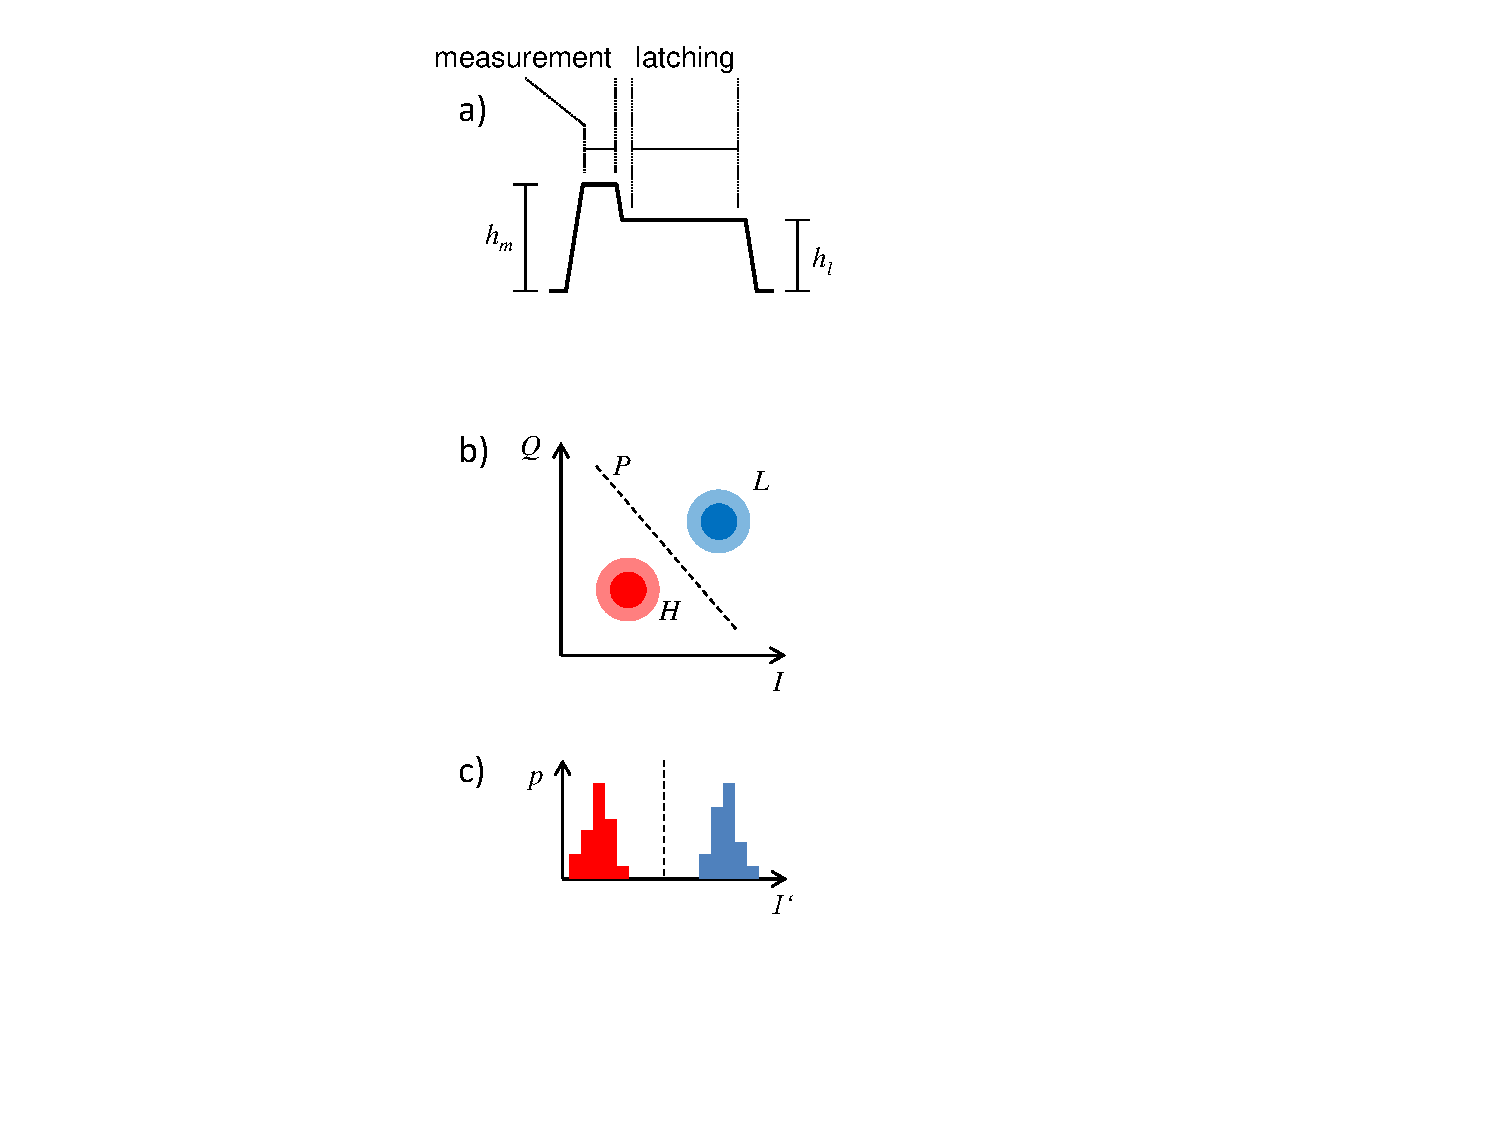
\includegraphics[width=\textwidth]{./material/figures/measurement/readout}
\caption[]{a) Microwave pulse envelope used for exciting the CJBA at readout.The pulse consists of a measurement part with amplitude $h_m$ and a latching part with amplitude $h_l=0.8-0.9h_m$. To determine the state of the resonator during the latching interval, the quadratures I and Q of the reflected signal are averaged over the time window $t_m$. b) Bimodal distribution of the time-averaged $(I,Q)$ values obtained for a readout power close to the bifurcation threshold . The red dotted line perpendicular to the principal axis joining the two modes of the distribution and going through the mean quadratures $(I_0,Q_0)$ provides an optimal separation between the two clusters corresponding to the L and H states. c) Histograms of the signal projected on the principal axis (red line), revealing a switching probability of 84\% for the  example shown.}
\label{fig:readout_bringup}
\end{figure}

The general principle of the CJBA readout used in this work is described in section \ref{section:cjba}. Here we explain how we choose its frequency $f_d$ and drive amplitude $a_d$. To bring up the readout, we first determine by reflectometry the resonance frequency $f_r$ of the CJBA in its linear regime, with the qubit in state $\ket{0}$ and largely detuned from the resonator. We then choose a relative drive detuning $\Omega=2Q(f_d/f_r-1)>\sqrt{3}$  (between 2 and 10 in practice, i.e. between 12 and 60 MHz ) at which the bistable regime is accessible. The continuous drive tone at $f_d$ is then split on two lines, one of them being mixed with the dc envelope coming from the AWG and sketched on fig. \ref{fig:readout_bringup}a. We then attenuate the resulting drive signal using a tunable attenuator at room temperature and send it to the CJBA. The reflected and amplified signal is then demodulated with the continuous drive present on the second line after the splitter, using an IQ demodulator. The resulting I/Q quadratures are further amplified, low-pass filtered at 200 MHz, and get digitized by the ADC card at a sampling rate of 1 GSample/s during the time window $t_m=1-2\mu$s sketched in fig. \ref{fig:readout_bringup}a. The digitized I/Q signals are then averaged over the whole measurement window to obtain a single measurement point in the IQ plane.  This sequence is repeated a large number of times (typically $10^4$) to obtain a statistical distribution of IQ points. We then repeat this procedure for various values of the input attenuation, each time calculating the estimated variance $\hat{\sigma}_{IQ}^2=\sum\limits_i ((I_i-\bar{I}_i)^2+\sum\limits_i (Q_i-\bar{Q}_i)^2)/n$ of the distribution. When starting with a high attenuation and reducing it, the input power sent to the CJBA will at some point be sufficient to make it switch from the L to the H state, thereby changing the phase and consequently the I and Q average values of the distribution. Since the switching is a stochastic process, we will observe two distinct sets of points close to the transition power. At an input power where approximately 50 \% of switching occurs, the variance $\sigma_{IQ}^2$ of the obtained IQ data points will be largest, as shown in fig. \ref{fig:readout_bringup}b. At this point, we subtract the averages $(I_0=\sum\limits_i I_i / n,Q_0 = \sum\limits_i Q_i/n)$ from the data and perform a principal axis transformation, which diagonalizes their covariance matrix
%
\begin{equation}
\mathrm{var}_{IQ} = \left(\begin{array}{cc}\mathrm{var}(I) & \mathrm{cov}(I,Q) \\ \mathrm{cov}(I,Q) & \mathrm{var}(Q) \end{array}\right).
\end{equation}
%

\begin{SCfigure}[1][hb!]
\centering
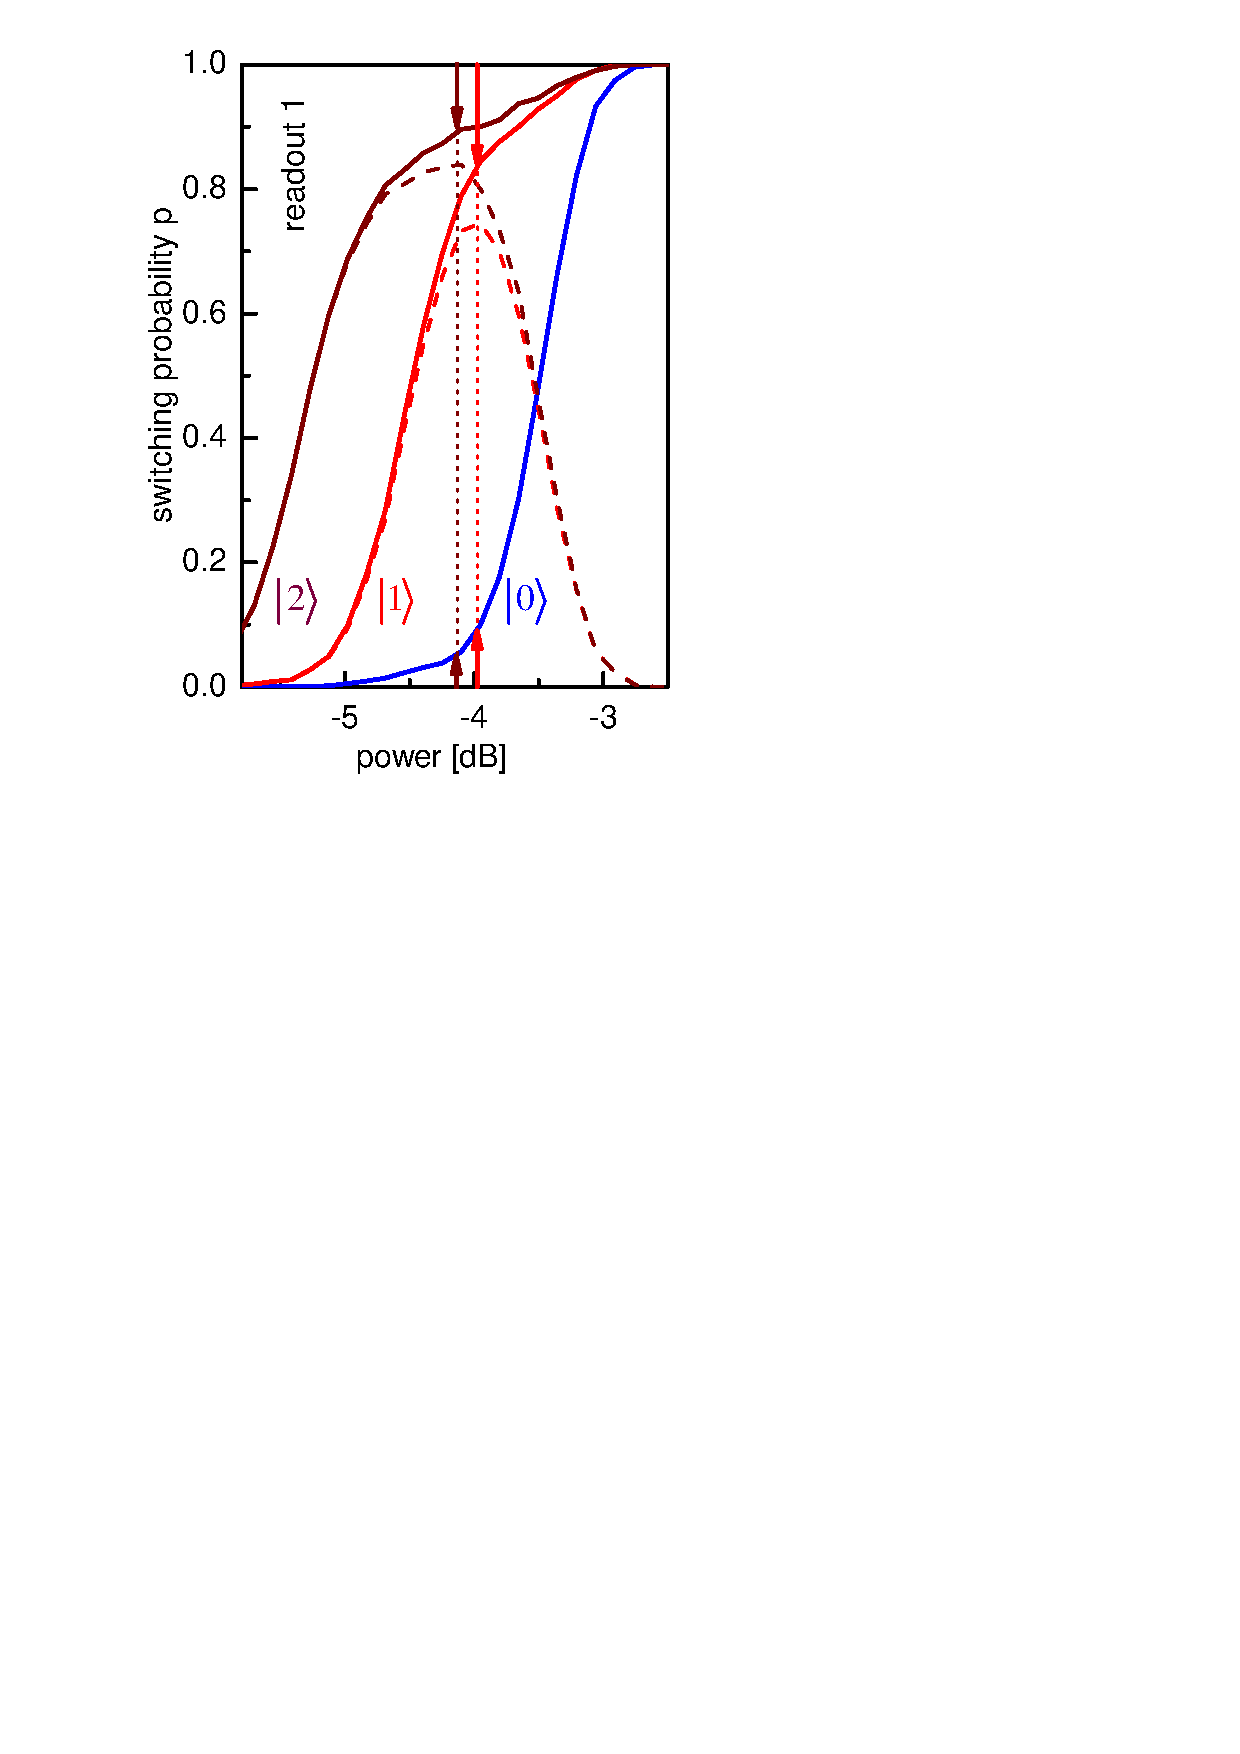
\includegraphics[width=0.4\textwidth]{./material/papers/grover/figures/s_curves_example}
\caption{Exemplary S-curve measured for one of the qubit-readout. Shown is the switching probability $p$ of the CJBA as a function of the readout signal power, plotted for the different qubit states $\ket{0}$,$\ket{1}$ and $\ket{2}$. The readout contrast between different states is given as difference between the associated switching probability curves. Light and dark red arrows indicate the optimal working points where the $c_{01}$ and $c_{02}$ readout contrasts are maximum, respectively.}
\label{fig:s_curves_example}
\end{SCfigure}

Using this transformation, we project the measured (I,Q) points on the axis $\perp P$ joining the two sub-distribution, as shown in fig. \ref{fig:readout_bringup}, and obtain a bivalued one-dimensional probability distribution. Then, the obtained offsets $I_0$, $Q_0$ and principal axis rotation angle $\alpha_{IQ}$ gives us the discrimination criterion $Q_L<Q_0+\tan{\alpha_{IQ}}(I-I_0)$ used to classify new data points as belonging to the L or H state at the chosen working point. Normally, if the measurement window $t_m$ is large enough and no retrapping occurs during the measurement, the distributions corresponding to the L and H states do not overlap, yielding perfect discrimination between them, as shown on the figure.

\smallskip

After having determined the $I_0$, $Q_0$ and $\alpha_{IQ}$, we slightly tune the attenuation to obtain $\approx 20\%$  of switching. At this working point, the readout contrast of the CJBA is usually already sufficient to perform a simple qubit spectroscopy, as described in section \ref{section:qubit_spectroscopy} and calibrate a $X_\pi$ Rabi pulse, as described in section \ref{section:qubit_rabi}. After having done this, we calibrate and optimize each qubit readout by measuring the switching probability as a function of the input power while either leaving the qubit in state $\ket{0}$ or exciting it to the state $\ket{1}$. Fig. \ref{fig:s_curves_example} shows an example of such a measurement. Here, the difference $c_{01}$ between the two curves corresponding to the $\ket{1}$ and $\ket{0}$ states defines the input-power dependent readout contrast. The optimal  input power chosen for reading the qubit out is where the contrast is maximum. If desired, we use instead a $X_\pi^{12}\cdot X_\pi^{10}$ pulse sequence to bring the qubit into state $\ket{2}$ before readout. In this state, the dispersive shift of the resonator frequency is larger then in the state $\ket{1}$, therefore resulting in a larger readout contrast $\mathrm{max}(c_{02})>\mathrm{max}(c_{01})$, as shown in fig. \ref{fig:s_curves_example}. This shelving of state $\ket{1}$ to state $\ket{2}$ is advantageous when performing e.g. single-run quantum algorithms on the processor, as described in chapter \ref{chapter:grover_algorithm}.

\subsection{Qubit Spectroscopy} \label{section:qubit_spectroscopy}

\begin{SCfigure}[1.0][ht!]
\begin{tabular}{l}
a) \\ \includegraphics[width=0.55\textwidth]{"./material/figures/measurement/qubit_spectroscopy"} \\
b) \\ \includegraphics[width=0.6\textwidth]{"./data/ct5/2011_04_21 - grover and tomo/example - qubit 2 spectroscopy"} \\
\end{tabular}
\caption[]{a) Qubit drive and readout pulse sequence used for qubit spectroscopy. b) Example of qubit spectrum showing the switching probability of the qubit readout when driving the qubit with 1 $\mu$s-long pulse as a function of the drive frequency. Low power spectroscopy (red points) shows only the $\ket{0}\to\ket{1}$ transition of the qubit at frequency $f_{01}$, whereas the 2-photon $\ket{0}\to\ket{2}$ transition at frequency $f_{02}/2$ is also observed at higher power (blue points). Lorentzian functions (lines) are fitted to these two spectroscopic lines.}
\label{fig:qubit_spectroscopy_example}
\end{SCfigure}

In order to characterize the transition frequency and anharmonicity of the qubit we perform spectroscopic measurements. For this we drive the qubit with a long Rabi pulse (usually $> 1\;\mathrm{\mu}$s) at a frequency $\omega_d$. When the drive frequency $\omega_{d}$ is close to the $\omega_{01}$ frequency of the qubit, the drive pulse will induce a Rabi oscillation of the quantum state of the qubit. The induced rotation amplitude will be largest at $\omega_d=\omega_{01}$. Due to decoherence during the driven evolution, the maximum probability for measuring the qubit in the state $\ket{1}$ at the end of the pulse will be limited to 50 \%. By repeating the pulse sequence shown in fig. \ref{fig:qubit_spectroscopy_example}a for a range of drive frequencies $\omega_d$, a full spectroscopy of the qubit can be obtained. Fig. \ref{fig:qubit_spectroscopy_example}b shows an example of this, for different drive amplitudes. Here, the blue curve has been measured at $10\;\mathrm{dB}$ higher power then the red curve, which is sufficient to observe the two-photon $\ket{0}\to\ket{2}$ transition of the qubit at $f_{02}/2$. By fitting the two resonance curves with a Lorentzian model we obtain the qubit frequencies $f_{01}$ and $f_{02}/2$, and from the equations of section \ref{section:transmon_qubit}, the charging and Josephson energies of the qubit at the given working point.

\subsection{Rabi Oscillations} \label{section:qubit_rabi}

\begin{SCfigure}[1.0][ht!]
\begin{tabular}{l}
a) \\ \includegraphics[width=0.55\textwidth]{"./material/figures/measurement/qubit_rabi_oscillation"} \\
b) \\ \includegraphics[width=0.6\textwidth]{"./data/ct5/2011_04_21 - grover and tomo/example - qubit 2 rabi"} \\
\end{tabular}
\caption[]{a) Qubit drive and readout pulse sequence used for measuring Rabi oscillations. b) Example of a measured Rabi oscillation showing the switching probability of the qubit readout when driving the qubit at $f_{01}$ with a Gaussian drive pulse of increasing effective duration t (points). The measurement results are not corrected for readout errors. The line is a fit by an exponentially decaying sine function. The grey dashed line shows the measurement data corrected for readout errors.}
\label{fig:qubit_rabi_example}
\end{SCfigure}

After having obtained the proper qubit transition frequency $f_{01}$, we calibrate Rabi pulses. For this, we  perform a Rabi oscillation experiment that consists in driving the qubit at $f_{01} $with pulses of increasing areas and in measuring its state immediately afterwards. Figure \ref{fig:qubit_rabi_example} shows the pulse sequence that we use and the resulting measurement data, the readout switching probability being expressed as a function of an equivalent pulse length at a nominal pulse height. As can be seen, the amplitude of the Rabi oscillations gets damped as  $p(t)=p_0+{\Delta}p\cos{(\Omega t)}\exp{(-\Gamma_R t)}$ due to relaxation and dephasing during the driven evolution. Also, the maximum readout contrast is limited due to readout errors characterized in details in the next chapter. From the fit of the Rabi data we obtain the Rabi frequency $\Omega$, which we use to program precise single-qubit rotations in all our experimental sequences. Note that due to the finite anharmonicity of the qubit, there is always a finite leakage to the second excited state $\ket{2}$, which we discuss later.

\subsection{Relaxation Time Measurement}

\begin{SCfigure}[1.0][ht!]
\begin{tabular}{l}
a) \\ \includegraphics[width=0.55\textwidth]{"./material/figures/measurement/qubit_t1_measurement"} \\
b) \\ \includegraphics[width=0.6\textwidth]{"./data/ct5/2011_04_21 - grover and tomo/example - qubit 2 t1"} \\
\end{tabular}
\caption[]{a) Qubit drive and readout pulse sequence used for relaxation time measurement. b) Example of relaxation time measurement showing the probability of measuring the qubit in state $\ket{1}$ as a function of the delay time between the preparation of the state $\ket{1}$ and the actual measurement of the qubit state (points). The line is a fit by a decaying exponential. The grey dashed line shows the measurement data corrected for readout errors.}
\label{fig:qubit_t1_example}
\end{SCfigure}

Having obtained the transition frequency $f_{01}$ and calibrated the Rabi frequency $\Omega$, we measure the relaxation time of the qubit. For this, we put the qubit in state $\ket{1}$ by applying a $X_{\pi}$ pulse and let it evolve freely afterwards for a given delay time before reading out its state, as shown in fig. \ref{fig:qubit_t1_example}a. As can be seen on fig. \ref{fig:qubit_t1_example}b, the probability decreases exponentially as a function of time. A fit of the function $p(\ket{1}) = p_0+p_a\exp{(-\Gamma_1 t)}$ to the data yields the qubit relaxation rate $\Gamma_1$ at the given working point. In the following chapter we measure in more detail the relaxation time of both qubits as a function of their transition frequency and their detuning from the readout resonator.

\subsection{Dephasing Time Measurement}

\begin{SCfigure}[1.0][ht!]
\begin{tabular}{l}
a) \\ \includegraphics[width=0.55\textwidth]{"./material/figures/measurement/qubit_ramsey_oscillation"} \\
b) \\ \includegraphics[width=0.6\textwidth]{"./data/ct5/2011_04_21 - grover and tomo/example - qubit 2 ramsey"} \\
\end{tabular}
\caption[]{a) Qubit drive and readout pulse sequence used in a Ramsey experiment. (b) Example of a measured qubit Ramsey experiment showing the switching probability of the qubit readout (points) at the end of the sequence. Fitting the resulting curve with an attenuated sine-wave model (line) yields the dephasing rate $\Gamma_{\phi}$ and the qubit frequency $f_{01}$ (see text). The grey dashed line shows the measurement data corrected for readout errors.}
\label{fig:qubit_ramsey_example}
\end{SCfigure}

We also characterize the dephasing of each qubit by performing a so-called {\it Ramsey fringe experiment}, consisting in two $Y_{-\pi/2}$ pulses separated by a delay time ${\Delta}t$ and a readout immediately afterwards, as illustrated  on Fig. \ref{fig:qubit_ramsey_example}a. We either choose microwave pulses detuned from $f_{01}$ by an amount ${\Delta}f$, or use resonant microwave pulses together with a flux pulse that shifts the qubit frequency by ${\Delta}f$ during the whole delay. After the first pulse the qubit is in state $1/\sqrt{2}(\ket{0}+\ket{1})$ and acquires  a phase  $\Delta \phi = 2\pi\Delta f \Delta t$ during the delay. The final state of the qubit after applying the second $Y_{\pi/2}$ pulse therefore becomes
%
\begin{equation}
\ket{\phi_f} =1/\sqrt{2} \left(\begin{array}{cc} 1 & 1 \\ 1 & -1 \end{array} \right)\cdot\left(\begin{array}{c} 1 \\ e^{i\Delta\phi} \end{array}\right) = \left( \begin{array}{c}  -\cos{\Delta\phi/2} \\ i\sin{\Delta\phi/2} \end{array}\right),
\end{equation}
%
and the probability $p=\cos^2{\Delta\phi/2}$ to measure state $\ket{1}$ oscillates with frequency $\Delta f$ as a function of the delay ${\Delta}t$ . Due to dephasing and relaxation during the free evolution, the amplitude of these oscillations will decay. As explained in section \ref{section:decoherence_of_the_transmon}, this decay takes the form $\exp{(-\Gamma_2 t)}$ with $\Gamma_2=\Gamma_1/2 +\Gamma_{\phi}$ if the noise responsible for dephasing is white at low frequency, or the form $\exp{(-\Gamma_1 t/2 )}\exp{(-B t^2)}$ if the noise has a 1/f dependance. Even if the main dephasing source is 1/f flux noise of microscopic origin, the decay of the Ramsey oscillations is close to an exponential due to the relaxation contribution. So in practice, we fit the Ramsey data by $a cos({\Delta}f.t)\exp{(-\Gamma_2 t)}$ and deduce an effective dephasing rate $\Gamma_{\phi}$.
Furthermore, the fit provides an accurate measurement of ${\Delta}f$ and consequently of the qubit frequency $f_{01}$, which is now known with a precision of $100\;\mathrm{kHz}$. 
